%% ---------------- Hubo Walking in 5 days ------------------------
\chapter{Hubo Dynamic Walking - Developed in 5 Days Using Hubo-Ach}\label{sec:dynamicWalking}
Fig.~\ref{fig:dynamicwalking} shows Hubo2+ dynamic walking using Hubo-Ach as the primary controller.  The standard ZMP walking algorithms were implemented by our partners Mike Sillman and Matt Zucker at Geortia Gech and Swarthmore respectively.  All control was implemented using Daniel M. Lofaro's Hubo-Ach system.

\begin{figure}[thpb]
  \centering
  %\begin{tikzpicture}
    %\clip [rounded corners=1em] (0,0) rectangle coordinate (centerpoint) (5,7.5cm);
%    \node[minimum width=\linewidth,minimum height=174pt,draw=black,rounded corners=1em,fill=bgcolor,draw=black]
%    {};
%    \node[name=img] {
      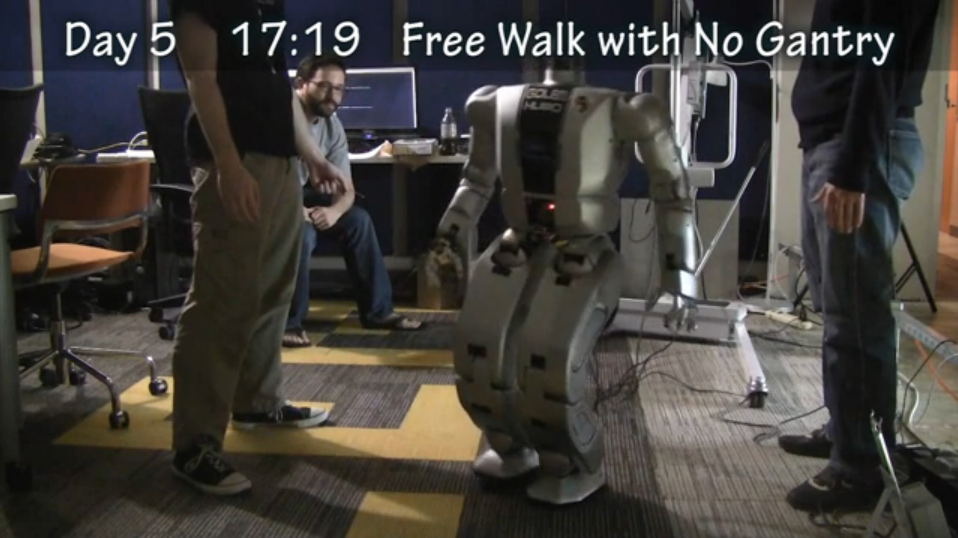
\includegraphics[width=0.6\columnwidth]{./examples/pix/dynamicwalking.png}
      
\includegraphics[width=0.3\columnwidth]{./qrcode/qrcode-dynamicwalking.png}\\
      Video: http://danlofaro.com/phd/walking/\#Walking5Days
%    };
%    \draw [bgcolor, rounded corners=1em, line width=1em,inner sep=0pt]
%    (img.north west) --
%    (img.north east) --
%    (img.south east) --
%    (img.south west) -- cycle
%    ;
%  \end{tikzpicture}
\caption{Hubo dynamic walking using Hubo-Ach as the primary controller.  The standard ZMP walking algorithms were implemented by our partners Mike Sillman and Matt Zucker at Geortia Gech and Swarthmore respectively.  All control was implemented using Daniel M. Lofaro's Hubo-Ach system.}
  \label{fig:dynamicwalking}
\end{figure}